
\chapter{Background: algorithmic tools for molecule discovery}
\label{chapter:background}

\ifpdf
    \graphicspath{{chapter02-background/figures}}
\else
    \graphicspath{}
\fi

This chapter provides a general overview of existing approaches to molecule discovery.
This is an incredibly large field with an enormous body of prior work
from chemistry, cheminformatics, and machine learning---
far too much to cover exhaustively.
Therefore, this chapter primarily aims to introduce the concepts and methods which
are necessary to understand the later chapters.
A brief summary of the chapter is provided at the end (\S\ref{sec:background:summary}).
Readers who are already familiar with the field may wish to skip directly to this summary
and then proceed to Chapter~\ref{chapter:lso}.

\section{Molecules and their representations}
\label{sec:background:mols}

The question ``what is a molecule'' is surprisingly nuanced and hard to answer
(see \S\ref{sec:what are molecules}).
All algorithms in this thesis interact with molecules only via some \emph{representation},
and therefore we denote by $\molspace$ the space of molecule representations.
Since the distinction between molecules and their representations
is not critical in this thesis, $\molspace$ will equivalently be referred to as simply
the space of molecules.\footnote{
    A more rigorous definition is as follows:
    let $\mathfrak{M}$ denote some abstract space of molecules,
    and let $r:\mathfrak M\mapsto \mathcal X$ map molecules to some representation
    space $\mathcal X$ with an equivalence relation.
    Define an equivalence relation $\sim$ between molecules by $m_1\sim m_2$ if
    $r(m_1)=r(m_2)$.
    $\molspace$ is then the quotient space $\mathfrak M / \sim$.
}

The fundamental representation used in this thesis is
\emph{standardized graphs}:
a set of nodes representing atoms and a set edges representing bonds between them.
Nodes possess a small set of discrete labels including atom type, electric charge,
and stereochemistry tags.\footnote{
    \citet[page~960]{zumdahl2006chemistry}
    defines \emph{stereoisomerism} as
    \begin{quote}
        where all the bonds in the isomers are the same but the spatial arrangements of the atoms are different.
    \end{quote}
    The general term ``stereochemistry tags'' is used in this thesis to refer to information
    used to disambiguate between stereoisomers.
    The exact specification of these tags is not important to the key ideas of this thesis,
    we simply emphasize that they exist.
}
Edges possess labels indicating bond types.
Examples of molecules are shown in Figure~\ref{fig:background-example-molecules}.
The \emph{standardization} refers to the resolution of a small number of equivalences between molecular graphs,
chiefly multiple ways of denoting bonds in aromatic rings.
The precise details of this standardization are not important to the key ideas of this thesis;
in practice it is delegated to third-party python packages.

\begin{figure}
    \centering
    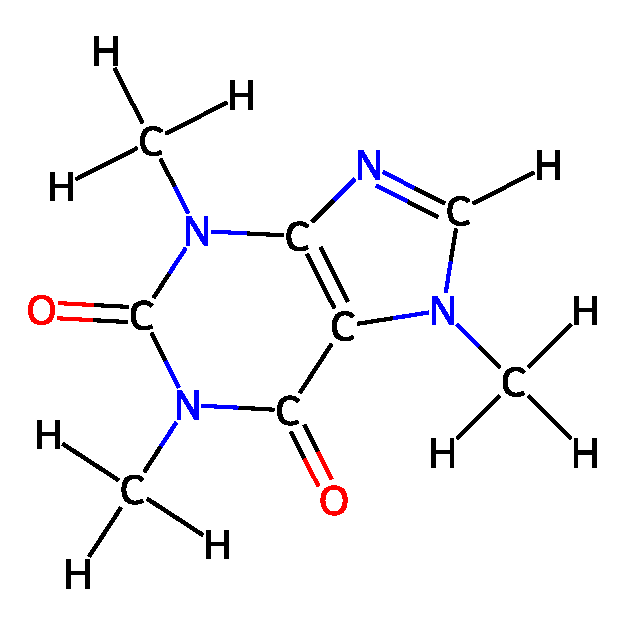
\includegraphics[width=0.4\textwidth]{caffeine-withHs.pdf}
    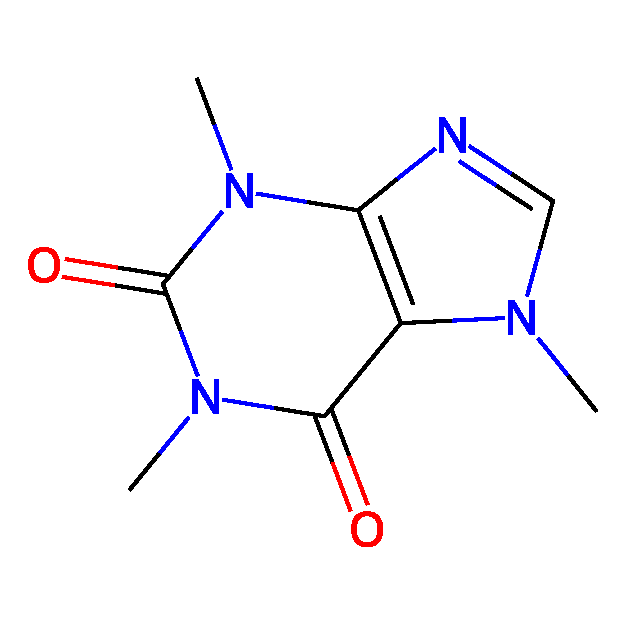
\includegraphics[width=0.4\textwidth]{caffeine-noHs.pdf}
    \caption[Graph of caffeine molecule.]{
        Left: graph for the molecule caffeine.
        Right: the \emph{skeletal formula} of the same graph:
        a simplified representation of the molecule which omits hydrogen atoms
        (whose presence can be inferred from the valency of the other atoms)
        and implicitly includes carbon atoms at the end of lines.
        Non-carbon atoms are labelled explicitly.
        This representation will be used in the remainder of the thesis.
    }
    \label{fig:background-example-molecules}
\end{figure}

With the exception of stereochemistry labels,
note that this representation excludes 3D descriptors of molecular structure,
despite molecules fundamentally being 3D objects.
This choice is made because in many practical applications one lacks both knowledge and control of a molecule's 3D structure
(the structure is determined by physics and the nanoscopic size of molecules preclude directly observing it).
Even when 3D structures can be inferred, the inability to freely \emph{control}
a molecule's 3D structure means this information is better viewed as a value calculated from the representation
rather than a fundamental property of the representation itself.

Note that for some problems,
only a subset of $\molspace$ is of interest.
In this case, we define $\amolspace\subseteq\molspace$ to be the set of \emph{accessible}
molecules for a given problem.
The exact nature of $\amolspace$ will be unique to each problem,
but could for example represent molecules which are purchasable
or molecules synthesizable within a fixed number of steps.
Many algorithms presented in this thesis are agnostic to the exact definition
of $\amolspace$ and it will therefore not be defined beyond simply being a subset of $\molspace$.
More specific definitions $\amolspace$ will be given when appropriate,
but should be understood to apply only within that specific section or chapter.

Although standardized graphs can sometimes be used directly as inputs to algorithms
(e.g.\@ in the form of a node list and an adjacency matrix),
it is often useful to post-process
these graphs into secondary, downstream representations
which are either not graph-structured or which yield additional information.
The remainder of this section will therefore introduce
common representations derived from graphs.
A more comprehensive introduction can be found in numerous review articles
\citep{david2020molecular,wigh2022representation,mcgibbon2023smol-representation}.

\subsection{Vector-valued \emph{descriptors}}

A molecular ``descriptor'' typically refers to some kind of real or integer quantity which can be computed from a graph.
Examples of simple descriptors are the number of atoms in a molecule,
the number of rotatable bonds, or the number of rings.
As of the writing of this thesis, the popular python package \texttt{rdkit}
provides over 200 structural descriptors of varying complexity.\footnote{
    See Greg Landrum's \href{https://greglandrum.github.io/rdkit-blog/posts/2022-12-23-descriptor-tutorial.html}{blog post from 2022-12-23}
    for details.
}
These descriptors can be selected and concatenated to form a fixed-length
vector representation of a molecule. 
Such representations were arguably more popular when machine learning was dominated by hand-engineered features,
and more broadly can be used when chemists' domain knowledge is sufficient to extract meaningful features for a given task.
However, this is not usually the case, and therefore such descriptors tend to be used only for naive baselines
and for heuristics such as ``Lipinski's rule of five'' \citep{lipinski2001experimental}.

\subsection{Vector-valued \emph{embeddings}}

Another approach to represent molecules as fixed-length vectors is to use the output of
machine learning models, most commonly neural networks.
We call such representations \emph{embeddings}.
Deferring the introduction of potential embedding models to \S\ref{sec:background:deep learning for molecules},
embeddings can be abstractly viewed as the output of functions $f_{\bm{\theta}}:\molspace\mapsto\R^m$
with parameters $\bm{\theta}$.
In principle there is no difference between embeddings and the ``descriptors''
introduced previously (both are vectors in $\R^m$).
However, in practice embeddings require model selection,
and unlike descriptor vectors individual dimensions of embeddings do not have a straightforward interpretation.
For this reason subsequent chapters will distinguish ``embedding'' vectors from ``descriptor'' vectors.

\subsection{String representations}
\label{sec:background:string-reps}

Any representation of molecules as sequence of discrete ``tokens'' (e.g.\@ letters of the alphabet)
can be considered a \emph{string representation}.
At present, the most popular and well-established string representation is unquestionably SMILES.
At a high level, a SMILES representation of a molecule marks a continuous ``path'' through a molecule
along bonded atoms, using parentheses `()' to denote branches from the path and numbers
to mark ring closures.
A simple example of a SMILES string is shown in Figure~\ref{fig:smiles-example}.
Because converting molecular graphs to/from SMILES representations
is handled by third-party python packages,
the precise details of SMILES syntax is not important in the context of this thesis
(although it is explained in more detail by \citet{weininger1988smiles}).
Only a few properties are important to understand subsequent material in this thesis:
\begin{enumerate}
    \item SMILES strings are formed from a fixed set of tokens,
        but not all arrangements of these tokens form a valid SMILES string.
        This sometimes necessitates ``validity checks''.
    \item Molecules can have multiple associated SMILES strings,
        which are formed by traversing a molecule's atoms in a different order.
        However, each SMILES string corresponds to only one graph.
        Therefore, the relationship between SMILES and graphs is a ``many to one'' mapping.
    \item It is possible to define \emph{canonical} SMILES such that there is a one-to-one relationship between molecular graphs and canonical SMILES.
        Algorithms to canonicalize SMILES are included in third-party libraries.
        This allows for collections of molecules to be stored as a set of canonical SMILES.
\end{enumerate}

\begin{figure}
    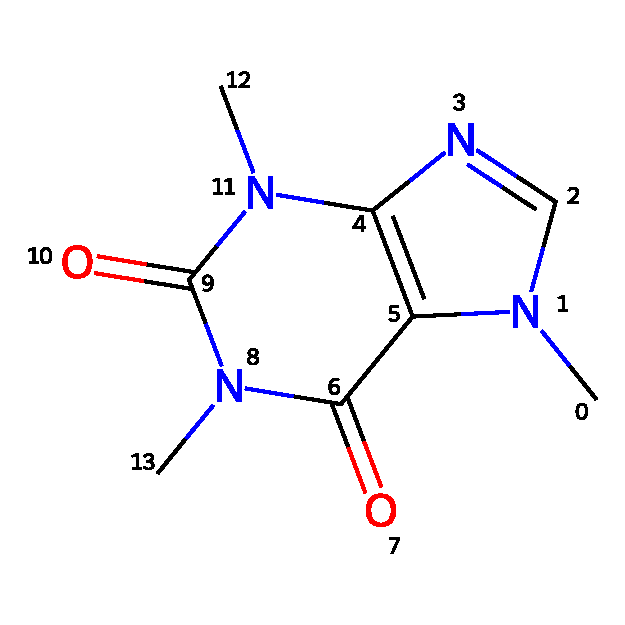
\includegraphics[width=0.4\textwidth]{caffeine-atom-indices.pdf}
    \begin{minipage}[b][0.4\textwidth][c]{0.55\textwidth}
        \begin{center}
            \begin{equation*}
                \setlength\arraycolsep{0pt}
                \begin{array}{cccccccccccccccccccccccccccc}
                        \texttt{C} & \texttt{N} & \texttt{1} & \texttt{C} & \texttt{=} & \texttt{N} & \texttt{C} & \texttt{2} & \texttt{=} & \texttt{C} & \texttt{1} & \texttt{C} & \texttt{(} & \texttt{=} & \texttt{O} & \texttt{)} & \texttt{N} & \texttt{(} & \texttt{C} & \texttt{(} & \texttt{=} & \texttt{O} & \texttt{)} & \texttt{N} & \texttt{2} & \texttt{C} & \texttt{)} & \texttt{C} \\
                        0          &      1     &            &          2 &            &          3 &     4      &            &            & 5          &            & 6          &            &            & 7          &            & 8          &            &       9    &            &            &     10     &            & 11         &            &  12        &            & 13
                    \end{array}
            \end{equation*}
        \end{center}
    \end{minipage}
    \caption[Explanation of SMILES string for caffeine]{
        Explanation of SMILES string for caffeine.
        The graph structure of caffeine is shown on the left, with all (non-hydrogen) atoms given an index.
        The SMILES string for caffeine is shown on the right.
        The numbers beneath each character indicate the corresponding atom index.
        Roughly, the string is formed by starting at atom $0$, traversing the right-hand ring to atom 5,
        then traversing the left hand ring to atom 12, and finally to the branching atom 13.
    }
    \label{fig:smiles-example}
\end{figure}

Other string representations exist to handle shortcomings of SMILES strings.
International Chemical Identifier (InChI) strings are more standardized
and use a hierarchical encoding to embed optional metadata such as stereochemistry tags,
but are not easy for humans to parse \citep{heller2015inchi}.
SELFIES are designed so that every arrangement of tokens from their alphabet forms a valid molecule
\citep{krenn2020self,krenn2022selfies}.
However, neither of these additional properties are useful for the works presented in this thesis,
thus these alternative representations are not used.

More generally, one may wonder why one would bother representing molecules as strings instead of graphs
given that such representations not only add no new information beyond the connectivity,
but arguably \emph{obscure} the graph connectivity.
In my opinion, the most principled reason is to allow molecules to be stored and processed
using simple data structures present in all programming languages.
For example, checking whether a molecule is present in a list of molecules can be done with a single line of python code
using string representations, avoiding any need for custom data structures or hash functions.
In contrast, I am not aware of any programming language with a built-in data structure for graphs.
However, probably the most important reason is to allow models and code for text data to be easily re-purposed for molecules.
I am sympathetic to the purist perspective this is an awkward, unprincipled contortion of a problem
just to fit the assumptions a conveniently-available method.
Admittedly however, the natural language processing community is much larger than the cheminformatics community,
and therefore has not only produced many methods to choose from,
but also fast and highly-optimised implementations of those methods that can be quickly deployed at a large scale.
Because speed is sometimes the most important factor for success,
I believe nonetheless that string representations have a place in machine learning for molecules.

\subsection{Molecular Fingerprints: a unifying perspective}
\label{sec:background:fingerprints}

Molecular fingerprints are possibly both the most commonly used
and the most commonly misunderstood molecular representation.
They are often described as fixed-length binary vectors
which encode a molecule's structure, produced by any number of different algorithms
\citep{yang2022concepts-fingerprint}.
Although this description does correctly describe the most common way in which fingerprints are used,
it does not apply to all fingerprints and overlooks clear similarities between fingerprint types.\footnote{
    My gripe with this view of fingerprints is that it seems to give many practitioners a misleading impression
    of the pros/cons to fingerprints.
    During informal conversations, other researchers have claimed to me that
    fingerprints are always binary, unavoidably high-dimensional,
    and unavoidably prone to ``collisions'' (where one dimension is assigned to multiple distinct substructures).
    Examining the default fingerprint objects in \texttt{rdkit} easily shows that all these claims are false.
    Hence, I think a better explanation of fingerprints is needed in the community.
}
My preferred, broader definition is as follows:

\begin{quotation}
    A molecular fingerprint is a multi-set of subgraphs present in a molecule,
    \emph{or} a post-processed derivative of such a multi-set.
\end{quotation}

The differences between the plethora of different fingerprinting algorithms used in prior work
can be succinctly summarized as either choosing different subgraphs for inclusion in the multi-set
or post-processing the multi-set in a different way.
Importantly, the multi-set construction and post-processing steps are conceptually separate
and can generally be chosen freely and combined as desired.
Therefore, we discuss them separately below.

\subsubsection{Constructing a multi-set of subgraphs}

Perhaps the simplest way of constructing a multi-set is to only include subgraphs from a pre-defined collection.
\citet{yang2022concepts-fingerprint}
refer to these as \emph{dictionary-based} fingerprints and
identify MACCS fingerprints as a prominent example.\footnote{
    MACCS fingerprints index 166 fragments including ``three-member ring'', ``CN'', or ``aromatic atom''.
    A full list can be found at: \url{https://github.com/rdkit/rdkit/blob/master/rdkit/Chem/MACCSkeys.py}
}
Other fingerprinting algorithms include subgraphs which correspond to \emph{paths} within a molecule.
These are referred to as \emph{topological fingerprints} by \citet{yang2022concepts-fingerprint}.
A popular example is \emph{atom-pair fingerprints}, which include shortest-path subgraphs between every pair of atoms
\citep{carhart1985atom}.

However, the most popular fingerprint seen in machine learning papers is ostensibly the \emph{extended-connectivity fingerprint},
also referred to as the \emph{Morgan fingerprint}.
\label{definition:morgan-fingerprint}
These fingerprints are characterized by an integer ``radius'' parameter,
and include subgraphs for every individual atom ($r=0$),
every atom with all its immediate neighbours ($r=1$), every atom with all immediate neighbours and all neighbours of neighbours ($r=2$), and so forth
up to some terminal radius $R$.
$R$ is typically chosen to be between $1$ and $4$.
These fingerprints are also referred to as ``circular fingerprints'' by \citet{yang2022concepts-fingerprint}
because they include ``circles'' of constant radius around each atom.
Subgraphs present in multiple locations are included multiple times in the multi-set.
An illustration of Morgan fingerprints is given in Figure~\ref{fig:morgan-fp-example}.
Other types of fingerprints will not be discussed here,
but interested readers can consult reviews on this topic for further discussion
\citep{cereto2015molecular,yang2022concepts-fingerprint}.

\begin{figure}
    \begin{minipage}[c]{0.06\textwidth}
        Atom 0%
        \\~\\~\\~\\~\\~\\~\\  %
        Atom 11
    \end{minipage}
    \begin{minipage}{0.22\textwidth}
        \centering
        $R=0$

        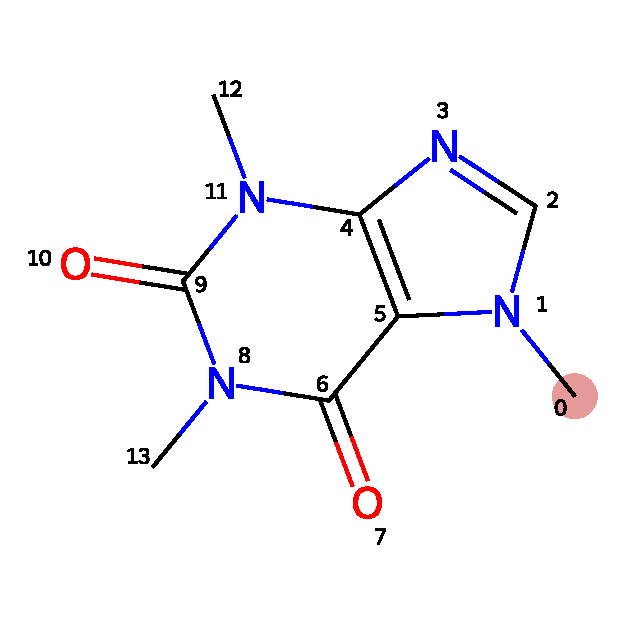
\includegraphics[width=\textwidth]{caffeine-atom0-fp0.pdf}
        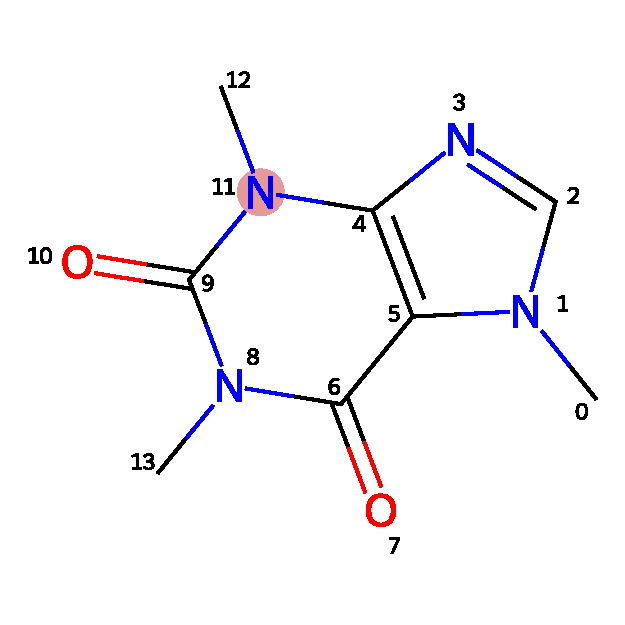
\includegraphics[width=\textwidth]{caffeine-atom11-fp0.pdf}
    \end{minipage}
    \begin{minipage}{0.22\textwidth}
        \centering
        $R=1$

        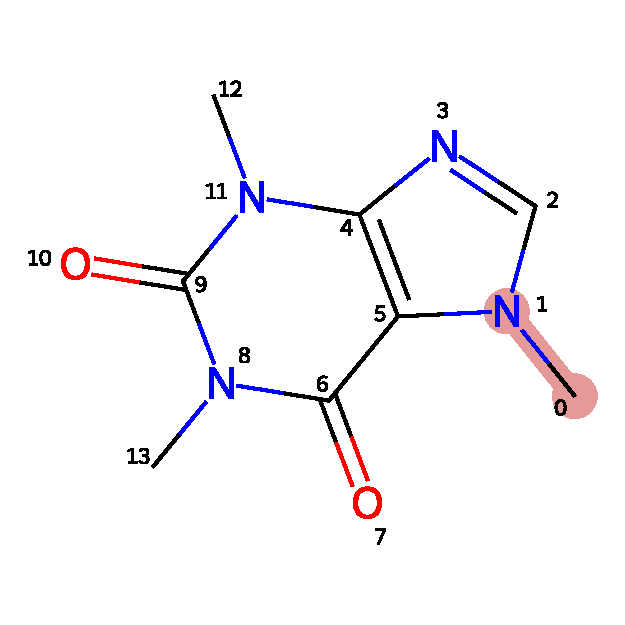
\includegraphics[width=\textwidth]{caffeine-atom0-fp1.pdf}
        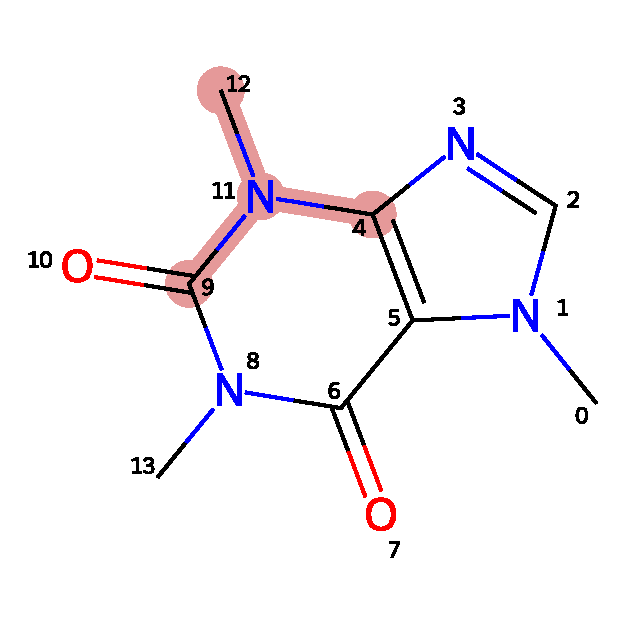
\includegraphics[width=\textwidth]{caffeine-atom11-fp1.pdf}
    \end{minipage}
    \begin{minipage}{0.22\textwidth}
        \centering
        $R=2$

        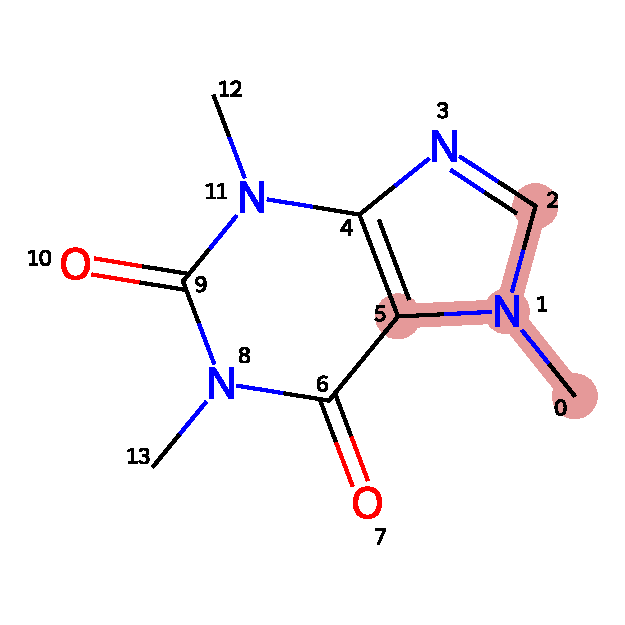
\includegraphics[width=\textwidth]{caffeine-atom0-fp2.pdf}
        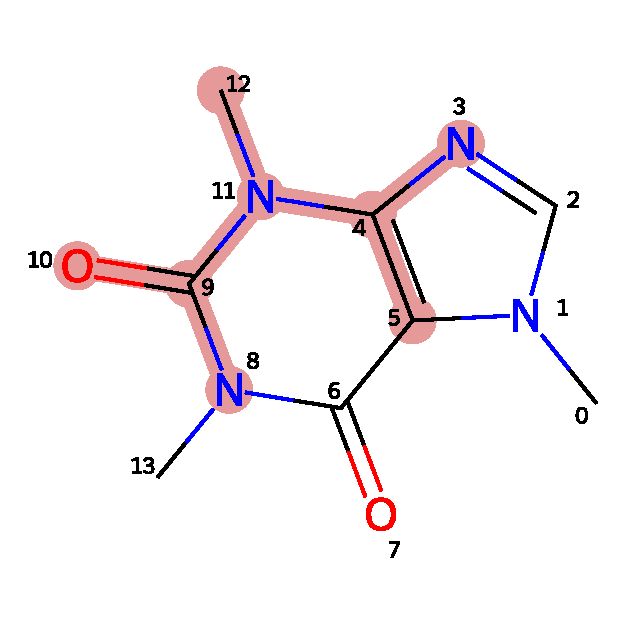
\includegraphics[width=\textwidth]{caffeine-atom11-fp2.pdf}
    \end{minipage}
    \begin{minipage}{0.22\textwidth}
        \centering
        $R=3$

        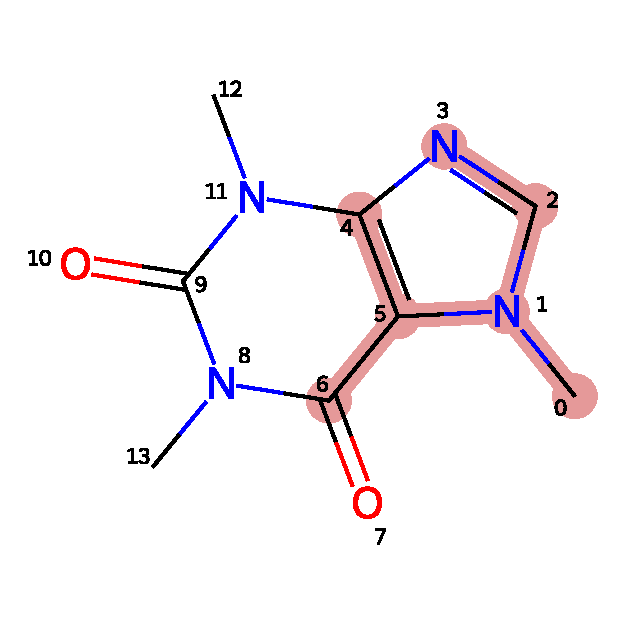
\includegraphics[width=\textwidth]{caffeine-atom0-fp3.pdf}
        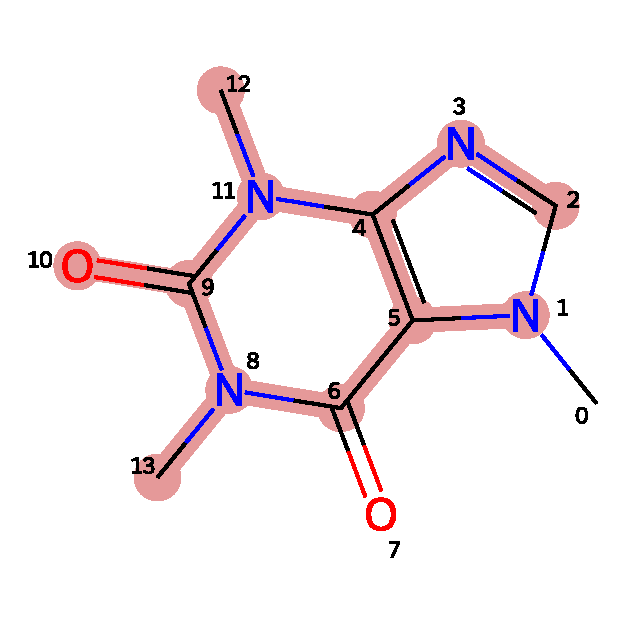
\includegraphics[width=\textwidth]{caffeine-atom11-fp3.pdf}
    \end{minipage}
    \caption[Illustration of subgraphs in Morgan fingerprints.]{
        Illustration of subgraphs of radius $0$ to $3$ around two atoms in caffeine
        (the carbon at index $0$ and the nitrogen at index $11$).
        Morgan fingerprints of radius $R=3$ would typically include the union of all such subgraphs
        for \emph{all atoms} (not just atoms $0$ and $11$) for \emph{all radii} from $0$ to $3$ (inclusive).
    }
    \label{fig:morgan-fp-example}
\end{figure}

\subsubsection{Post-processing multi-sets of subgraphs}

Post-processing consists of modifying the multi-set
and (optionally) converting the multi-set into a sparse vector.
The simplest kind of post-processing is the identity operator:
the multi-set is not modified, just returned as is.
Other common operations include discarding duplicate elements (thereby converting the multi-set into a plain set),
merging similar elements,\footnote{For example, paths with identical length and terminal atoms in atom-pair fingerprints.}
modifying elements,\footnote{For example, some implementations of Morgan fingerprints mask the identifies of the outermost ring of atoms to only consider the number of outgoing bonds.}
or deleting elements.\footnote{For example, some implementations of Morgan fingerprints effectively delete the $r=0$ subgraphs which consist of single atoms.}
After these modifications, the fingerprint can optionally be returned as a set-valued fingerprint.
Alternatively, to convert a fingerprint into a $k$-dimensional vector,
a hash function is first used to convert each subgraph in the multi-set to an integer in $\{1,\ldots,k\}$,
effectively forming a multi-set of integers $F$.
Then,
letting $\1_{\text{condition}}$ denote the indicator function (which is $1$ if the condition is true and $0$ otherwise),
a $k$-dimensional vector $v$ is formed such that
\begin{equation*}
    v_i=\1_{ i \in F }  
\end{equation*}
(referred to as a \emph{binary} fingerprint)
or
\begin{equation*}
    v_i=\sum_{j\in F} \1_{i = j}
\end{equation*}
(referred to as a \emph{count} fingerprint).
Note that count fingerprints differ from binary fingerprints only in the value of the non-zero indices
but not their location.
The vector $v$ is then returned as the fingerprint.

\subsubsection{Implementations of fingerprints}

In practice, implementations of fingerprinting algorithms may omit or combine certain steps for efficiency.
For example, most implementations of Morgan fingerprints directly compute hashes of subgraphs instead of forming
an explicit set of subgraphs.
Throughout this thesis fingerprint computations are handled by the third-party \texttt{rdkit} library
which computes Morgan fingerprint vectors of arbitrary length and radius (using an internal hash function).
Ultimately, only the following properties will be relied upon in subsequent chapters:
\begin{enumerate}
    \item Since the main difference between fingerprints is the set of subgraphs indexed, the ``type'' of most fingerprints is the same.
        Therefore, algorithms can be largely agnostic to the exact kind of fingerprint used.
    \item Fingerprints can be post-processed into vectors of different lengths and types, meaning that different versions of the same fingerprint can exist
        (e.g.\@ binary and count fingerprints).
        One can freely convert between these versions given the original set-valued fingerprint.
        This conversion is sometimes done implicitly.
    \item Fingerprints are not (necessarily) unique. For example, two molecules with the same atom count may have the same Morgan fingerprint of radius $0$.
        Therefore, in general, one cannot recover a molecule from its fingerprint.
\end{enumerate}

\section{Formulating molecular discovery problems}
\label{sec:background:problems}

Section~\ref{sec:intro:what is discovery}
linked ``discovery'' of a molecule to the measurement of one or more properties of interest.
Here we define these properties more precisely and discuss mathematical objectives which arise from this.

The most basic type of property is the real-valued property,
which can be represented as a function
$f:\molspace\mapsto\R$.
Nearly all physicochemical properties are real-valued, for example
solubility in water (e.g.\@ measured in $\mathrm{g\,L^{-1}}$),
binding energy to a protein (e.g.\@ measured in $\mathrm{kJ\,mol^{-1}}$),
electronic band gap (e.g.\@ measured in $\mathrm{eV}$),
or pH (a dimensionless quantity).
Many application-specific properties are also naturally real-valued,
for example the power conversion efficiency of an organic solar cell molecule (measured in \%),
or clinical outcomes of a drug molecule (e.g.\@ fraction of patients cured).

However, it is also necessary to consider categorical properties,
which can be represented as functions $f:\molspace\mapsto\{1,\ldots,C\}$ for some constant $C$
($C=2$ represents the special case of binary classification).
There are a small number of properties which are truly categorical,
for example whether a molecule contains a certain element
or whether a molecule is chiral.
However, most categorical properties originate from discretizing or aggregating real-valued properties.
For example, a drug molecule may be considered ``active'' if it has any non-negligible therapeutic outcome
(regardless of the intensity of that outcome),
otherwise inactive.
Another example is toxicity: a molecule may be considered ``toxic'' if it causes any number of adverse effects
at any intensity level.
Although such categorical properties are usually less fundamental than real-world properties,
they may nonetheless be useful in situations where observation noise is high
or when a discrete decision must be taken (e.g.\@ whether or not to disqualify a drug candidate due to toxic side effects).
In practice, many molecular datasets commonly seen in machine learning papers have categorical labels.

The following subsections describe the most common problems which
can be formulated from such property functions.

\subsection{Molecule optimisation and its variants}
\label{sec:background:molopt}

Given a space of accessible molecules $\amolspace\subseteq\molspace$
and a function $f:\molspace\mapsto\R$, \emph{molecule optimisation}
is the problem of finding
\begin{equation}\label{eqn:defn:molopt}
    m^* = \argmax_{m\in\amolspace} f(m) \quad,
\end{equation}
namely finding a molecule which maximises $f$.
This formulation makes sense when, all else being equal, one desires the \emph{best} molecule.
For example, if $f$ represents increase the increase in cancer survival rate caused by ingesting $m$
or power conversion efficiency of $m$ in a solar cell,
higher values of $f$ are undoubtedly better (assuming all other factors are held constant).

Equation~\ref{eqn:defn:molopt} is best viewed as defining the \emph{base} problem of molecule optimisation.
Variants of the problem can be categorized along the following (largely orthogonal) axes.

\subsubsection{Variation 1: Constraints}

As the phrase ``all else being equal'' highlights,
one is rarely just interested in maximising a single function.
For example, a drug molecule should not be toxic
or too expensive to produce,
and
an organic photovoltaic material must not degrade too quickly when exposed to sunlight.
These secondary interests can be formalized as constraints
on other property functions $f_1,f_2,\ldots$.
If a function $f_i$ is categorical then a constraint would usually take the form
$f_i(m)=c$,
whereas constraints for real-valued functions will usually take the form
$f_j(m)\in (a, b)$ (i.e.\@ lies within a certain interval).

However, in practice these constraints can often be incorporated into the base problem (equation~\ref{eqn:defn:molopt})
and not dealt with explicitly.
When constraints are known or easy to evaluate,
the set of accessible molecules $\amolspace$ can simply be re-defined to exclude any molecules which violate constraints.\footnote{
For example, if $\amolspace$ is originally a set of commercially purchasable molecules
and a constraint is that the molecular weight (MW) must be under 500 $\mathrm{g\,mol^{-1}}$,
$\amolspace$ can simply be redefined as $\amolspace' := \amolspace\cap\{m\,:\,m\in\molspace,\mathrm{MW}(m)<500\}$.
}
Alternatively, the constraints can be ``softened'' by adding a penalty for their violation
into the optimisation objective.\footnote{
For example, using the same molecular weight constraint as above,
one could re-define $f$ to be $f'(m) := f(m) + \lambda \max(\mathrm{MW}(m)-500, 0)$,
where $\lambda\in(0,\infty)$ controls the strength of the penalty.
}

Overall, because constraints can be incorporated into the base problem,
optimisation problems with constraints are not explicitly studied in this thesis.
Nonetheless, we mention constraints explicitly in order to clarify
that methods in this thesis are only not applicable to highly-idealized unconstrained problems.

\subsubsection{Variation 2: Knowledge of $f$}

Although it is hard to quantify, ``knowledge'' of the function $f$
greatly influences the difficulty of optimisation.
For example, if 
\begin{equation*}
    f(m) = \left| \mathrm{MW}(m) - a \right|\ ,
\end{equation*}
namely the distance between a molecule's
molecular weight and some target molecular weight $a$,
it is simple to reason about the function and optimise it
without actually doing experiments.
On the other hand, if $f$ is the percentage of cancer cells killed by a molecule,
then it is much harder to reason about the function $f$ because
it depends on many complex and poorly-understood interactions between
the molecule and the body.

In practice, we tend to know very little about the most interesting functions $f$.
Therefore, it is common to treat $f$ as a \emph{black-box} function,
meaning the function is only known by its input-output pairs.
In particular, this means one has no analytic expression for the function which can be exploited,
no significant knowledge of global properties like Lipschitz constants,\footnote{
    Technically, given a dataset of molecules and measurements
    one can always compute a \emph{lower bound} on the Lipschitz constant.
    However, if even a single pair of similar molecules have different properties
    then this lower bound can potentially be very large.
    Furthermore, as it is just a lower bound,
    it may not be very useful if one cannot rule out the possibility
    of the actual Lipschitz constant being much larger.
}
and no knowledge of local information such as gradients (not that gradients are applicable to molecules anyway).
Less strict formulations such as grey-box optimisation have also been considered in other works,
but will not be studied in this thesis.

\subsubsection{Variation 3: Noise and measurement error}

In laboratories, properties of molecules are measured with imperfect machines
in a somewhat uncontrolled environment
operated by humans who may make mistakes.
This means that one does not generally have access to ``true'' evaluations of $f$:
instead, one acquires a noisy measurement $y$,
which can contain both random error (i.e.\@ repeating the same measurement will give different outcomes)
and systematic error (i.e.\@ averaging repeated measurements may not converge to $f(m)$).
This can be formalized as $y=f(m)+\epsilon$
where $\epsilon$ is a random variable which can depend on $m$ and may have a non-zero mean.
In practice however, a common assumption is that $\epsilon$ is normally distributed with
mean zero and variance $\sigma^2$.

\subsubsection{Variation 4: Data availability and acquisition}

If one can perform unlimited evaluations of $f$ then optimisation is a trivial problem
which can be tackled with exhaustive search.
In practice, evaluating $f$ is too costly or time-consuming to permit exhaustive evaluation.
Therefore, molecule optimisation problems are dominated by their access to data.
This access to data comes in two forms.
First, before optimisation a dataset of molecules and measurements
$\mathcal{D}=\{(m_i,y_i)\}_{i=1}^N$
is available.
Second, during optimisation the algorithm will be able to acquire labels for at most $B$
data points.
We refer to $B$ as the evaluation \emph{budget}.
Optimisation algorithms will typically iterate between choosing a molecule
and making a measurement until the budget is exhausted.

This evaluation strategy is sometimes called \emph{sequential evaluation},
in contrast to \emph{batch evaluation} wherein multiple evaluations are made simultaneously.
Batch evaluation is very common in chemistry since many scientific instruments
readily 
support parallel measurements:
for example, spectrometers commonly measure optical absorptions of ``plate''
of 96 liquid samples simultaneously.
However, given a fixed budget, optimisation with batch evaluation is generally more
challenging than with sequential evaluation.
This is because one must commit to a large number of experiments upfront
before seeing any results,
while in the sequential setting the results of every experiment can be used to improve
decisions at each step.

\subsubsection{Variation 5: Measuring success}

Naively, one might think to evaluate a molecule optimisation
algorithm by checking whether it finds the true $\argmax$ in equation~\ref{eqn:defn:molopt}.
Sadly this is infeasible since $\max_m{f(m)}$ is almost always unknown,
and even if it where known it is unlikely that many algorithms
would find it given a sufficiently small budget $B$.
Not knowing $\max_m{f(m)}$ also precludes using regret as a metric,
which is popular choice for many theoretical optimisation works.
Finally, given that one only has access to noisy measurements $y$ of $f$,
a success metric must only depend on measurements.

Because of this, the most sensible metrics in molecule optimisation
are the cumulative measurement value $$\sum_{i=1}^B y_i\ ,$$
the maximum measurement value $$\displaystyle \max_{i\in\{1,\ldots,B\}}y_i\ ,$$
or its generalization to the $k$th-best measurement value (also referred to as \emph{top-k}).
The top-k metric is arguably the most realistic for many discovery settings
where the goal is to find a small number of promising molecules.
However, because it depends only on a small number of measurements
it is also sensitive to measurement noise and randomness in the optimisation algorithm used.
In this regard, the cumulative measurement value is more stable.


\subsection{Supervised Learning}
\label{sec:background:supervised learning}

Let $\mathcal X$ denote an input space (e.g.\@ $\R^n$ or $\molspace$)
and $\mathcal Y$ denote an output space (e.g.\@ $\R$ or $\{1,\ldots,C\}$).
Supervised learning is the problem of directly approximating a property function $f:\mathcal X\mapsto \mathcal Y$
with some \emph{surrogate model} $\hat{f}$.
Although producing a surrogate model does not directly discover molecules,
an accurate surrogate model could clearly be used to select promising molecules
from a pre-defined list or to guide a more general molecule optimisation algorithm (\S\ref{sec:background:molopt}).
In this thesis two variants of supervised learning are considered.

\subsubsection{Single-Task Learning}

This is the standard setting where a single model $\hat{f}$
is produced to approximate labels (measurements) from a single dataset
$\mathcal{D}:=\{(m_i,y_i)\}_{i=1}^N$.
The model is typically produced to minimise a \emph{loss function}
$\mathcal{L}(\hat f, \mathcal D)$ on $\mathcal D$.
Examples of loss functions include misclassification error (for classification problems),
mean squared error (for regression problems),
or negative marginal likelihood (for probabilistic models).

\subsubsection{Multi-task / Meta-learning Learning}

In this setting a \emph{collection} of datasets $\{\mathcal D_1, \ldots, \mathcal D_M \}$
is provided, and the goal is to produce a corresponding collection
of models $\{\hat f_1, \ldots, \hat f_M\}$.
It is essentially just multiple instances of single-task learning problems,
and one approach is to produce a completely independent model for each dataset.
However, this setting is also amenable to approaches wherein
the models $\hat f_1, \ldots, \hat f_M$ are \emph{not} independent,
for example they may share parameters.

\section{Probabilistic models for molecular properties}
\label{sec:background:models}

The main contributions presented in this thesis are algorithms which \emph{use}
models to perform supervised learning (\S\ref{sec:background:supervised learning})
or molecule optimisation (\S\ref{sec:background:molopt}),
while being mostly agnostic to the details of the models themselves.
Furthermore, since molecules can be represented as sequences and vectors (\S\ref{sec:background:mols}),
and since these data types are arguably the most studied data types in all of machine learning,
there exists an enormous number of machine learning models which \emph{could} be applied to molecules.
Therefore, this section will not even attempt to present a comprehensive introduction to such methods;
if interested a reader may consult any number of high-quality textbooks or reviews
\citep{bishop2006pattern,Goodfellow-et-al-2016deep-learning,murphy2022probabilistic}.
Instead, this section will present and contextualize a small number of model classes which appear in this thesis,
and will also explain their probabilistic interpretation (which may not be familiar to all readers).

\subsection{Probabilistic linear models}
\label{sec:background:linear models}

Given a \emph{feature} function $\phi:\mathcal X \mapsto \R^M$,
linear regression defines $\hat f: \mathcal X \mapsto \R$ as
\begin{equation}
    \hat f (x) = \bm{w} \cdot \phi (x) + b \quad .
\end{equation}
This model has a vector of \emph{weight} parameters $\bm{w}\in\R^M$
and a \emph{bias} parameter $b\in\R$.
In a non-probabilistic regression setting $\hat f$ is directly used to predict
labels $y$ (typically called ``linear regression'').
In the probabilistic setting however,
$\hat f$ is connected to $y$ via an \emph{observation model}
which assigns a probability to every possible outcome for $y$.

For regression, this observation model is most often
a Gaussian distribution centred on $\hat f(x)$,
with probability density function
\begin{equation}\label{eqn:background:gaussian noise}
    p_{\bm{w}, b, \sigma^2}(y|x) = \mathcal{N}(y; \hat f(x), \sigma^2)\quad .
\end{equation}
Here, $\mathcal N(y; a, b)$ is the probability density
of a Gaussian distribution with mean $a$
and variance (or covariance matrix) $b$ at $y$.
The parameter $\sigma^2$ is also called the \emph{noise} parameter.

For \emph{binary} classification ($C=2$),
the model
\begin{equation}
    \probability_{\bm{w}, b}\left(y=1|x\right) = \frac{e^{\hat f(x)}}{1 + e^{\hat f (x)}}
\end{equation}
is typically used ($\probability$ denotes the probability of an event).\footnote{
    This is also called \emph{logistic regression}.
}
For $C>2$ a single linear model is insufficient to assign probabilities to all outcomes;
instead a set of linear models with parameters $(\bm{w_1}, b_1),\ldots,(\bm{w}_C, b_C)$
is created, with
\begin{equation}
    \probability_{\bm{w}_1,b_1,\ldots,\bm{w}_C,b_C} \left( y = i | x \right) \propto e^{\hat f_i(x)}\quad .
\end{equation}

Linear models are not used directly in this thesis, but
form the basis for more complex models introduced in the following sections.

\subsection{Gaussian processes and Bayesian linear models}
\label{sec:background:gps}

The crux of Bayesian modelling is to treat the model itself as a random variable,
typically by introducing a \emph{prior} distribution on the model parameters.
If a standard normal $\mathcal N(\bm{0}, \mI)$ prior is put on the linear model weights
$\bm{w}$, this induces the distribution
\begin{equation}
    \begin{bmatrix}
        \hat f (x_1) \\
        \vdots \\
        \hat f (x_N)
    \end{bmatrix}
    \sim \mathcal N \left(b \bm{1}, \mK \right)
\end{equation}
over the outcomes $\hat f (x_1), \ldots, \hat f (x_N)$
(which are random variables by implication of $\bm{w}$ being a random variable).
Here, $\bm{1}$ denotes a vector of $1$s,
and $\mK$ is a matrix whose entries correspond to inner products between feature vectors
\begin{equation}\label{eqn:background:kernel function defn}
    \emK_{i,j}=k(x_i,x_j):=\phi(x_i) \cdot \phi(x_j) \quad .
\end{equation}

The function $k(\cdot, \cdot)$ is called the \emph{kernel function}
(discussed further in \S\ref{sec:background:mol-kernels}).
Because the distribution of $\hat f$ depends only on features $\phi$
via the inner product function $k$,
it is common to define Bayesian linear models directly using $k$.
In this context, such models are usually referred to as \emph{Gaussian processes} (GPs)
and can be thought of directly defining a distribution over functions $\mathcal X\mapsto \R$:
\begin{equation}
    \hat f \sim \mathcal{GP}(\mu(\cdot), k(\cdot, \cdot)) \quad .
\end{equation}

Measurements $y_1,\ldots,y_N$ can then be described as sampled from distributions
induced by random samples of $\hat f$.
However, what really makes GPs useful for machine learning is that
if the observation model is also Gaussian (equation~\ref{eqn:background:gaussian noise}),
then the Bayesian posterior distribution over $\hat f$ is \emph{also a Gaussian process}
(although with a different mean and kernel function which depend on the observed data).
With a constant noise value of $\sigma^2$, the posterior distribution over query points
$x^*_1, \ldots, x^*_Q$ 
given observations
$((x_1, y_1), \ldots (x_N, y_N))$
has the form
\begin{equation}
    \begin{bmatrix}
        \hat f(x^*_1) \\
        \vdots \\
        \hat f(x^*_Q)
    \end{bmatrix}
    \sim \mathcal{GP} \left(\tilde \mu (\cdot), \tilde k(\cdot, \cdot) \right)
\end{equation}
where
\begin{align}
    \tilde \mu(x^*) &= \mu(x^*) 
    + \begin{bmatrix}
        k(x^*, x_1) \\
        \vdots \\
        k(x^*, x_N)
    \end{bmatrix}^T
    \left(\mK(X, X) + \sigma^2\mI\right)^{-1}
    \begin{bmatrix}
        y_1 - \mu(x_1) \\
        \vdots \\
        y_N - \mu(x_N) \\
    \end{bmatrix}\quad,  \\
    \tilde k(x^*_i, x^*_j) &=
    k(x^*_i, x^*_j) -
    \begin{bmatrix}
        k(x^*_i, x_1) \\
        \vdots \\
        k(x^*_i, x_N)
    \end{bmatrix}^T
    \left(\mK(X, X) + \sigma^2\mI\right)^{-1}
    \begin{bmatrix}
        k(x_1, x^*_j) \\
        \vdots \\
        k(x_N, x^*_j)
    \end{bmatrix}\quad,  \\
    \mK(X,X)_{i,j} &= k(x_i,x_j)
\end{align}
\citep{rasmussen2006gp}.
This also allows the marginal likelihood of the data to be computed in closed form.
For a GP with a constant noise value $\sigma^2$,
mean function $\mu(\cdot)$, and kernel function $k(\cdot, \cdot)$,
the (log) marginal likelihood of the data $X=\left[x_1,\ldots,x_N\right]$
is given by
\begin{equation}\label{eqn:background:gp-marginal-likelihood}
    \log{p(\bm{y}|X)} =
        -\frac{1}{2}\bm{y}^T
            \left(\mK(X, X) + \sigma^2\mI\right)^{-1}
            \bm{y}
        -\frac{1}{2}\log\left|\mK(X, X) + \sigma^2\mI\right|
        -\frac{N}{2}\log(2\pi)
\end{equation}
\citep{rasmussen2006gp}.
GP models are often selected to maximise the marginal likelihood of the data
by maximising equation~\ref{eqn:background:gp-marginal-likelihood}
with respect to the parameters of the mean and kernel functions.
    
\subsection{Gaussian process kernels \emph{for molecules}}
\label{sec:background:mol-kernels}

Equation~\ref{eqn:background:kernel function defn}
defined the kernel function $k(\cdot, \cdot)$ as the inner product of feature vectors.
However, in practice it is much more common to define the kernel function directly.
Any kernel function which is \emph{positive definite}
(i.e.\@ no kernel matrix formed from the kernel function will have negative eigenvalues)
will implicitly correspond to an inner product between feature vectors
in some Hilbert space, which may be infinite-dimensional
\citep{scholkopf2002learning}.
Since the kernel provides the primary inductive bias of GP models,
it is important to choose a kernel function carefully.

For vector-valued data in $\R^n$,
the most common kernels are the \emph{radial basis function} (RBF) kernel
\begin{equation}\label{eqn:rfb kernel defn}
    k(x, x') = \exp\left(-\frac{\|x - x'\|^2}{2\ell^2}\right)
\end{equation}
or the \emph{Mat\'ern} family of kernels, indexed by a parameter $\nu$.
A common value for $\nu$ is $\nu=5/2$,
which yields the kernel function
\begin{equation}\label{eqn:matern52 kernel defn}
    k(x, x') = \left(1 + \frac{\sqrt{5}\|x - x'\|}{\ell} + \frac{5\|x - x'\|^2}{3\ell^2}\right)
    \exp\left(-\frac{\sqrt{5}\|x - x'\|}{\ell}\right) \quad .
\end{equation}
Both of these kernels encode the assumption that input vectors
with a small Euclidean distance are likely to have similar outputs.

Vector valued kernels can be applied to some molecular representations
(e.g.\@ embeddings) but are not directly applicable to molecular graphs.
For fingerprint representations of molecules it is useful to define set-valued kernels.
A notable set kernel which will be used in several places throughout this thesis is the
\emph{Tanimoto kernel},
also called the \emph{Jaccard kernel}
\citep{jaccard1912distribution,tanimoto1958elementary}.
This kernel has been widely used in cheminformatics to compare molecular fingerprints
\citep{ralaivola2005graph,bajusz2015tanimoto,o2016comparing,miranda2021differential}.
It can be defined in several equivalent ways.
For plain sets, the definition
\begin{equation}\label{eqn:background:tanimoto-for-sets}
    T(S_1, S_2) = \frac{\left| S_1 \cap S_2 \right|}{\left| S_1 \cup S_2 \right|}
\end{equation}
suffices.
This definition can easily be extended to multi-sets.
Letting $m_i(x)$ denote the multiplicity of $x$ in multi-set $S_i$,
we define
\begin{equation}\label{eqn:background:tanimoto-for-multisets}
    T(S_1, S_2) = \frac{\sum_{x\in S_1\cup S_2}\min\left(m_1(x), m_2(x)\right)}{\sum_{x\in S_1\cup S_2}\max\left(m_1(x), m_2(x)\right)} \hfill .
\end{equation}
Note that equations~\ref{eqn:background:tanimoto-for-sets} and \ref{eqn:background:tanimoto-for-multisets}
are consistent and compatible using standard notions of intersection/union for multi-sets.
This kernel encodes the inductive bias that input sets with a high degree of overlap
are likely to have similar outputs.
When applied to molecular fingerprints, this is equivalent to assuming
that molecules with similar substructures are likely to have similar properties.

The Tanimoto kernel has the useful property that $1-T(\cdot, \cdot)$ is a valid distance metric,
typically called the \emph{Jaccard/Soergel distance}
\citep{marczewski1958certain,levandowsky1971distance}.
This makes it useful in nearest-neighbour methods in addition to GP models
(although this will not be exploited in this thesis).

Combining the Tanimoto kernel with a molecular fingerprinting function
creates a kernel directly over graph space.
Prior works have also developed many other kernels 
which operate directly on graph-structured inputs 
\citep{nikolentzos2021graph}.
These kernels generally also perform some sort of comparison of substructures present within the two input graphs.
For example,
\citet{moss2020boss} converts graphs into SMILES strings and defines a kernel based on substring matching.
\citet{korovina2020chembo} proposes a kernel based on graph optimal transport.
These kernels are not used directly in this thesis and so will not be discussed further.


\subsection{Fast approximations for Gaussian processes}
\label{sec:background:approx-gp-inference}

Regardless of the kernel used, GP models are notorious for scaling poorly to large datasets.
Evaluating the posterior covariance requires computing the kernel value between all
pairs of input data in $x_1,\ldots,x_N$ (time complexity $\mathcal O (N^2)$)
and inverting a regularized version of this matrix (time complexity $\mathcal O (N^3)$).
Even if $N$ is small, producing a full covariance matrix between $Q$
query points still has $\mathcal O(Q^2)$ cost,
and many operations such as sampling require inverting this matrix ($\mathcal O(Q^3)$).
For this reason approximations to GPs have been widely studied
\citep{liu2020scalable-gps}.

There are many different approaches which all aim to avoid expensive matrix computations in different ways.
One popular class of approaches are \emph{inducing point methods}.
These approximate a GP over $x_1,\ldots,x_N$
with a GP over a smaller set of $M$ pseudo-data points $z_1,\ldots,z_M\in\mathcal X$.
If $M\ll N$ these approximations will be significantly faster than the exact GP,
generally reducing $\mathcal O (N^2)$ operations to $\mathcal O(MN)$ and $\mathcal O (N^2)$ to $O(NM^2)$.
The inducing points function as a set of tunable parameters
and are generally chosen to ``cover'' the dataset.
A commonly-used model of this type is the stochastic
variational Gaussian process (SVGP) 
\citep{titsias2009variational,hensman2013gaussian}.

Another approach is \emph{random features} \citep{rahimi2007random}.
Given a kernel $k$, a \emph{random features map} 
is a random function
$f:\mathcal{X}\mapsto\mathbb{R}^M$, with the property that  $f(x)\cdot f(x')$ approximates $k(x,x')$ for every pair $x,x'\in\mathcal X$.
The approximation is often exact in expectation:
\begin{equation}\label{eqn:random-feature-definition}
    \mathbb{E}_f\left[f(x)\cdot f(x')\right]=k(x,x') \quad \text{for all }x,x'\in\mathcal X.
\end{equation}
Random features effectively create a rank-$M$ approximation to the kernel matrix $\mK(\mX, \mY) \approx f(\mX)^T f(\mY)$.
This results in the same reductions to computational cost as the inducing point approximations,
i.e.\@ at most linear in $N$.
A random features map is sometimes called a \emph{data-oblivious sketch}, to distinguish it from other \emph{data-dependent}
low-rank approximation methods which depend on a given dataset.
Examples of data-dependent low rank sketches are the Nystr\"{o}m approximation and leverage-score sampling \citep{drineas2005nystrom,drineas2012fast}.
Although data-dependent methods may result in lower approximation errors for a given dataset,
data-oblivious sketches are naturally parallelizable and useful in cases where the dataset  changes over time (e.g.\@ streaming or optimisation)
or for ultra-large datasets which may not fit in memory.

Other approaches accept the $\mathcal O (N^2)$ construction of the kernel matrix,
but try to approximate its inversion in less than $\mathcal O (N^3)$ complexity.
Approaches in this category include conjugate gradient methods
\citep{gardner2018gpytorch,wang2019exact}
and stochastic gradient methods
\citep{antoran2023samplingbased,lin2023sampling-sgd,lin2024stochastic}.
However, these are not used in this thesis.

Importantly, note that these methods are ultimately \emph{approximations}
to exact Gaussian processes and therefore will in general provide different predictions.
Approximate GPs are best thought of as sacrificing prediction quality
for computational tractability.

\subsection{Deep Learning and Neural Networks}
\label{sec:background:deep learning for molecules}

Deep learning describes an enormous family of models which map inputs to outputs
using a sequence of non-linear transformations (typically differentiable).
Deep learning has proliferated enormously over the past decade,
producing a deluge of model types.
A thorough introduction to deep learning can be found elsewhere
\citep{Goodfellow-et-al-2016deep-learning,murphy2022probabilistic}.
Here we will only briefly mention the neural network types which are used in this thesis.

\begin{itemize}
    \item \textbf{Feedforward neural networks},
        also called a multi-layer perceptron (MLP) for historical reasons,
        transform vector inputs to vector outputs using an alternating sequence of matrix multiplications
        and non-linear transformations referred to as ``activation functions''.
        They are described in detail in \citet[chapter 6]{Goodfellow-et-al-2016deep-learning}.
    \item \textbf{Graph neural networks} (GNNs)
        accept graphs as inputs and produce vectors as outputs.
        Many GNNs effectively pass ``messages'' between nodes,
        which are weighted by learnable parameters to produce an embedding for each node.
        These embeddings are aggregated to produce an overall graph embedding.
        A more thorough introduction to GNNs is given in
        \citet{zhou2020graph}.
\end{itemize}

Throughout this thesis neural networks will simply be treated as parameterized
functions $f_{\bm{\theta}}:\molspace \mapsto \R^n$
whose outputs are differentiable with respect to the parameters $\bm{\theta}$.
The outputs of $f_{\bm{\theta}}$ can be used as the input features to a linear model
(\S\ref{sec:background:linear models}),
and thereby can form probabilistic models in the same way.


\section{Generative models for molecules}
\label{sec:background:molgen}

Estimates have suggested that as many as $10^{60}$ small organic molecules may exist
\citep{bohacek1996art},
yet even the largest chemical libraries contain only $\approx10^{20}$ molecules
\citep{hoffmann2019next}.
To cover a larger fraction of chemical space, it makes sense to represent chemical space \emph{implicitly}
using an algorithm to generate molecules.
There are many algorithms which can do this
\citep{xu2019deep,du2022molgensurvey}.
A notable type are \emph{generative models},
which (implicitly or explicitly) specify a distribution $p(m)$ over molecule space.
Here we briefly review some \emph{deep} generative models for molecules,
which use neural networks to define $p(m)$.

Since molecules are discrete objects with variable size,
deep generative models for molecules all tend to parameterize some
kind of iterative construction process to produce a molecule incrementally.
Recurrent neural networks and transformers define a distribution
for the next token given all the previous tokens
\citep{Goodfellow-et-al-2016deep-learning,turner2023introduction},
and can thereby be used to generate string representations of molecules
(\S\ref{sec:background:string-reps}).
Other, more complex models construct graph objects directly by adding one node at a time.
Examples of such architectures are the graph convolutional policy network \citep{you_graph_2018},
and the junction-tree decoder \citep{jin_junction_2019}.

All of these models can be used to perform unconditional generation by allowing
for some stochasticity when making choices of tokens to add.
They can also be modified to accept an additional vector input $\bm{z}$.
This allows them to be used in conditional deep generative models.
One popular such model is the variational autoencoder (VAE) \citep{kingma2013auto}.
VAEs treat $\bm{z}$ as a latent variable and introduce a prior $p(\bm{z})$ over it.
Because the resulting distribution $p_{\bm{\theta}}(x):=\int p_{\bm{\theta}}(x|\bm{z})p(\bm{z})\,d\bm{z}$
is intractable for high-dimensional $\bm{z}$,
VAEs instead introduce an approximate posterior $q_{\bm{\phi}}(\bm{z}|x)$
and maximise the variational lower bound
\begin{equation}
    \log{p_{\bm{\theta}}(x)} \geq
    \E_{\bm{z}\sim q_{\bm{\phi}}(\bm{z}|x)} \left[
        \log{p_{\bm{\theta}}(x|\bm{z})p(\bm{z})}
        - \log{q_{\bm{\phi}}(\bm{z}|x)}
    \right]
\end{equation}
with respect to the parameters $\bm{\theta},\bm{\phi}$.
This objective can be estimated by a mix of Monte-Carlo sampling and analytical expressions,
especially when $p(\bm{z})$ and $q_{\bm{\phi}}(\bm{z}|x)$ have a similar form (e.g.\@ both Gaussian).

Besides VAEs, other popular latent variable models are GANs \citep{goodfellow2014generative}
and normalizing flows \citep{rezende2014stochastic,papamakarios2021normalizing}.
However, their training is better suited for continuous data so they are less useful for molecules.

More recent works propose to generate molecules using diffusion models,
both in 3D \citep{yang2023diffusionmodels,hoogeboom2022equivariant,xu2022geodiff,jing2022torsional}
and 2D \citep{jo2022scorebased,vignac2023digress,liu2023generativediffusion,yang2023diffusionmodels}.
These models are arguably ``state of the art'' in all kinds of generative tasks
and may possibly be the best method for molecule generation.\footnote{
    However, as I recently argued in \citet{tripp2023genetic},
    simply generating valid molecular graphs is not very difficult,
    so it is hard to say whether diffusion models are actually better than other methods.
}
However, they will not be used in this thesis, chiefly because they did not exist
when my work on molecule generation in chapter~\ref{chapter:lso} was performed.

\section{Retrosynthetic planning (retrosynthesis)}
\label{sec:background:synthesis}

Performing a physical measurement on a molecule requires either purchasing it or producing it.
Given that even the largest databases of immediately purchasable molecules (such as Enamine) contain only $10^9$ compounds,
accessing most of chemical space requires producing molecules oneself.
This can be achieved by purchasing precursor molecules and performing one or more chemical reactions,
a process called \emph{synthesis}.

Not all molecules are easy to synthesize however, and previous work has shown that many molecules generated
by machine learning models are difficult to synthesize
\citep{gao2020synthesizability}.
If the space of synthesizable molecules is unknown,
this is equivalent to having an incomplete knowledge of
the space of accessible molecules $\amolspace$,
causing issues for molecular optimisation (\S\ref{sec:background:molopt}).
This motivates the importance of explicitly considering synthesis.

There are a few techniques to do this.
One is to produce some kind of ``synthesizability''
score for a molecule, which estimates how easy it is to synthesize.
Some models of this type include synthetic accessibility (SA) scores
\citep{ertl2009estimation},
SC score \citep{coley2018scscore},
and RA score \citep{thakkar2021retrosynthetic}.
Such scores are typically quick to compute,
but are not always accurate.\footnote{
    A fundamental problem with synthesizability scores
    is that ``synthesizability'' is not well-defined.
    Whether a molecule is ``synthesizable'' or not depends on
    ones resources, expertise, and time.
    A large pharmaceutical company will likely be able to synthesize
    more molecules than a lone graduate student.
}
Another technique is to generate synthesis plans directly,
for example using generative models
\citep{bradshaw2019model,bradshaw2020barking,gottipati2020learning,gao2021amortized}.
These models have the advantage of producing an explicit synthesis plan,
but the disadvantage of not having direct control over what molecule the synthesis plan produces!

Because of this, there is arguably no perfect substitute for explicit retrosynthetic planning:
creating a synthesis plan for a pre-specified target molecule by working backwards.
Retrosynthesis has a long history of automation in chemistry
\citep{vleduts1963concerning,corey1969computer}.
The rest of this section will discuss retrosynthetic planning.

\subsection{Problem definition}

Let $\rxnspace$ denote the space of single-product chemical reactions
which transform a set of \emph{reactant} molecules $R\subseteq\molspace$
into a
\emph{product} molecule in $\molspace$.
A large amount of work has been on training machine learning models
to predict reactant sets
which will produce a given product molecule
\citep{segler2017neural,dai2019retrosynthesis,%
seidl2021modern,chen2021deep,sacha2021molecule,irwin2022chemformer,%
zhong2022root,liu2023fusionretro}.
These models are trained on large datasets of known reactions.
The exact nature of these models is not important for the work presented in this thesis,
and therefore we will represent these models abstractly as
a \emph{backward reaction model} function $B:\gM\mapsto 2^\gR$.

The reactions predicted by a backward reaction model can be used to define
a \emph{reaction graph} $\gG$.
There are generally two kinds of reaction graphs.
The first type is called and AND/OR graph.
It is a directed graph which contains two types of nodes:
molecule nodes (also called OR nodes)
and reaction nodes (also called AND nodes).
Molecule nodes contain outgoing edges towards reactions which produce them,
and reaction nodes contain outgoing edges towards their reactant molecules.
Note that direction of the edges (from products towards reactants)
is the \emph{opposite} of how the reaction would actually be performed
(from reactants to products).
There are two subtypes of AND/OR graphs:
graphs which contain only one node for each molecule and each reaction
(and therefore may contain cycles if reversible reactions are present)
and graphs wherein these cycles are ``unrolled''.
We refer to the former type of search graph as simply a ``graph,''
while the latter type is called a ``tree.''
Examples of an AND/OR graph
and its corresponding
AND/OR tree are shown in Figure~\ref{fig:graphs-vs-trees-schematic}.

\begin{figure}[ht]
    \centering
    \begin{minipage}{.48\textwidth}
    \centering
    
    \begin{tikzpicture}[node distance=0.5cm]
          \node[ornode] (target) at (0, 0) {$\targetmol$};

          \node[andnode, below left = of target] (r1) {$r_1$};
          \draw[->] (target) -- (r1);
          \node[ornode, below = of r1] (ma) {$m_a$};
          \draw[->] (r1) -- (ma);
          
          \node[andnode, below = of ma] (r2) {$r_2$};
          \draw[->] (ma) -- (r2);
          \node[ornode, below = of r2] (mb) {$m_b$};
          \draw[->] (r2) -- (mb);

          \node[andnode, below right = of target] (r3) {$r_3$};
          \draw[->] (target) -- (r3);
          \node[ornode, below right = of r3] (mc) {$m_c$};
          \draw[->] (r3) -- (mc);

          \node[andnode, above = of mc] (r4) {$r_4$};
          \draw[->] (mc) -- (r4);
          \draw[->] (r4) -- (target);
    \end{tikzpicture}

    \vfill
    a) Graph version
\end{minipage}
\begin{minipage}{.48\textwidth}
    \centering
    \begin{tikzpicture}[node distance=0.5cm]
          \node[ornode] (target) at (0, 0) {$\targetmol$};

          \node[andnode, below left = of target] (r1) {$r_1$};
          \draw[->] (target) -- (r1);
          \node[ornode, below = of r1] (ma) {$m_a$};
          \draw[->] (r1) -- (ma);
          
          \node[andnode, below = of ma] (r2) {$r_2$};
          \draw[->] (ma) -- (r2);
          \node[ornode, below = of r2] (mb) {$m_b$};
          \draw[->] (r2) -- (mb);

          \node[andnode, below right = of target] (r3) {$r_3$};
          \draw[->] (target) -- (r3);
          \node[ornode, below = of r3] (mc) {$m_c$};
          \draw[->] (r3) -- (mc);

          \node[andnode, below = of mc] (r4) {$r_4$};
          \draw[->] (mc) -- (r4);
          \node[ornode, below = of r4] (target2) {$\targetmol$};
          \draw[->] (r4) -- (target2);
          \node[andnode, below = of target2] (r3-2) {$r_3$};
          \draw[->] (target2) -- (r3-2);
          \node[labelnode, below = of r3-2] (dots) {$\vdots$};
          \draw[->] (r3-2) -- (dots);
    \end{tikzpicture}

    b) Tree version

\end{minipage}

    \caption[Example of an AND/OR graph and tree.]{
        AND/OR graph and tree representation of the reaction set
        $\targetmol\Rightarrow m_a$ ($r_1$),
        $m_a\Rightarrow m_b$ ($r_2$),
        $\targetmol\Rightarrow m_c$ ($r_3$),
        and
        $m_c\Rightarrow \targetmol$ ($r_4$).
    }
    \label{fig:graphs-vs-trees-schematic}
\end{figure}

A second kind of reaction graph is an OR tree.
This is a directed graph where each node corresponds to a \emph{set}
of molecules,
and outgoing edges correspond to reactions which produce the set of molecules
from another set of molecules (not necessarily using all of the molecules as reactants though).
In this type of graph, cycles are always unrolled so that the graph is always a tree.
An example of an OR tree is shown in Figure~\ref{fig:or-graph-schematic}.

\begin{figure}[ht]
    \centering
    \begin{tikzpicture}[node distance=0.5cm]
      \node[ornode] (target) at (0, 0) {$\{\targetmol\}$};

      \node[ornode, below left = of target] (ma) {$\{m_a\}$};
      \draw[->] (target) -- (ma);
      
      \node[ornode, below = of ma] (mb) {$\{m_b\}$};
      \draw[->] (ma) -- (mb);

      \node[ornode, below right = of target] (mc) {$\{m_c\}$};
      \draw[->] (target) -- (mc);
      
      \node[ornode, below = of mc] (target2) {$\{\targetmol\}$};
      \draw[->] (mc) -- (target2);
      \node[ornode, below = of target2] (mc2) {$\{m_c\}$};
      \draw[->] (target2) -- (mc2);
      \node[labelnode, below = of mc2] (dots) {$\vdots$};
      \draw[->] (mc2) -- (dots);
\end{tikzpicture}

    \caption{OR tree for same set of reactions as Figure~\ref{fig:graphs-vs-trees-schematic}.}
    \label{fig:or-graph-schematic}
\end{figure}

One could imagine forming a ``complete'' reaction graph $\gG$ by starting with a
\emph{target molecule} $\targetmol$ and iteratively ``growing''
a graph by using a backward reaction model $B$ to add reactions
to all leaf molecules until no molecules remain.
This ``complete'' graph $\gG$ would contain all possible synthesis plans,
and therefore be a natural object for retrosynthetic planning.
Unfortunately, the size of this graph will typically grow exponentially
with the depth, and therefore be too large to compute in practice
(analogous to the game trees of chess and Go).
Instead, retrosynthetic planning will be performed
on an \emph{explicit search} $\gG'\subseteq\gG$.
In contrast, the ``complete'' graph $\gG$ will be called the \emph{implicit search graph}.

A \emph{synthesis plan} for a molecule $m$ is a sequence of chemical reactions
which produces $m$ as the final product.
Synthesis plans usually form trees $T\subseteq\gG$
(more generally directed acyclic subgraphs),
wherein each molecule is produced by at most one reaction.
The set of all synthesis plans in $\gG$ which produce a molecule $m$
is denoted $\enumplans_m(\gG)$.
Figure~\ref{fig:retrosynthesis-background-schematic} provides an example
of an explicit search graph (a) and all synthesis plans for $\targetmol$
which are contained within it (b).
Not all synthesis plans are equally useful however.
Most importantly,
for a synthesis plan to actually be executed by a chemist
the starting molecules must all be bought.
Typically this is formalized as requiring all starting molecules
to be contained in an \emph{inventory} $\gI\subseteq\molspace$.
It is also desirable for synthesis plans to have low cost,
fewer steps, and reactions which are easier to perform.

\begin{figure}[ht]
    \centering
    \begin{minipage}{.48\textwidth}
    \centering
    
    \begin{tikzpicture}[node distance=0.5cm]
          \node[ornode] (target) at (0, 0) {$\targetmol$};

          \node[andnode, below left = of target] (r1) {$r_1$};%
          \draw[->] (target) -- (r1);
          \node[ornode, below left = of r1] (ma) {$m_a$};
          \draw[->] (r1) -- (ma);
          \node[ornode, below right = of r1] (mb) {$m_b$};
          \draw[->] (r1) -- (mb);
          
          \node[andnode, below right = of target] (r2) {$r_2$};%
          \draw[->] (target) -- (r2);
          \draw[->] (r2) -- (mb);
          \node[ornode, below = of r2] (mc) {$m_c$};
          \draw[->] (r2) -- (mc);
          \node[ornode, below right = of r2] (md) {$m_d$};
          \draw[->] (r2) -- (md);
          
          \node[andnode, below = of ma] (r3) {$r_3$};%
          \draw[->] (ma) -- (r3);
          \node[ornode, below = of r3] (me) {$m_e$};
          \draw[->] (r3) -- (me);

          \node[andnode, below left = of mc] (rc1) {$r_4$};
          \draw[->] (mc) -- (rc1);
          \node[andnode, below right = of mc] (rc2) {$r_5$};
          \draw[->] (mc) -- (rc2);
          \node[ornode, below = of rc1] (mf) {$m_f$};
          \draw[->] (rc1) -- (mf);
          \node[ornode, below = of rc2] (mg) {$m_g$};
          \draw[->] (rc2) -- (mg);
          \node[draw, dashed, fit=(rc1) (rc2) (mf) (mg), inner sep=6pt, label=below:{expansion of $m_c$}] (box) {};
    \end{tikzpicture}

    \vfill
    a) $\gG'$
\end{minipage}
\begin{minipage}{.48\textwidth}
    \centering

    \begin{tikzpicture}[node distance=0.5cm]
        \node (T1) at (-1,0) {$T_1:$};
        \node[ornode] (target) at (0, 0) {$\targetmol$};
        
        \node (T2) at (-1,-1) {$T_2:$};
        \node[ornode] (target2) at (0, -1) {$\targetmol$};
        \node[andnode, right = of target2] (r1) {$r_1$};
        \draw[->] (target2) -- (r1);
        \node[ornode, above right = of r1] (ma) {$m_a$};
        \draw[->] (r1) -- (ma);
        \node[ornode, right = of r1] (mb) {$m_b$};
        \draw[->] (r1) -- (mb);
        
        \node (T3) at (-1,-2.2) {$T_3:$};
        \node[ornode] (target3) at (0, -2.2) {$\targetmol$};
        \node[andnode, right = of target3] (r1b) {$r_1$};
        \draw[->] (target3) -- (r1b);
        \node[ornode, right = of r1b] (mb2) {$m_b$};
        \draw[->] (r1b) -- (mb2);
        \node[ornode, above right = of mb2, xshift=-.2cm, yshift=-.2cm] (ma2) {$m_a$};
        \draw[->] (r1b) |- (ma2);
        \node[andnode, right = of ma2, xshift=-0.2cm] (r3) {$r_3$};
        \draw[->] (ma2) -- (r3);
        \node[ornode, right = of r3, xshift=-0.2cm] (me) {$m_e$};
        \draw[->] (r3) -- (me);

        \node (T4) at (-1,-3.5) {$T_4:$};
        \node[ornode] (target4) at (0, -3.5) {$\targetmol$};
        \node[andnode, right = of target4] (r2) {$r_2$};
        \draw[->] (target4) -- (r2);
        \node[ornode, right = of r2] (mc) {$m_c$};
        \draw[->] (r2) -- (mc);
        \node[ornode, above right = of mc, xshift=-0.2cm, yshift=-0.2cm] (mb) {$m_b$};
        \draw[->] (r2) |- (mb);
        \node[ornode, below right = of mc, , xshift=-0.2cm, yshift=+0.2cm] (md) {$m_d$};
        \draw[->] (r2) |- (md);

    \end{tikzpicture}

    b) $\enumplans_{\targetmol}\left(\gG'\right)$

\end{minipage}

    \caption[AND/OR graph and its synthesis plans.]{
       \textbf{a)} graph $\gG'$ with (backward) reactions
            $\targetmol\Rightarrow m_a+m_b\,(r_1)$,
            $\targetmol\Rightarrow m_b+m_c+m_d\,(r_2)$,
            and $m_a\Rightarrow m_e\,(r_3)$.
            Dashed box illustrates expansion of $m_c$. %
        \textbf{b)} All synthesis plans in $\enumplans_{\targetmol}(\gG')$.
    }
    \label{fig:retrosynthesis-background-schematic}
\end{figure}

Various search algorithms have been proposed to find synthesis plans in $\gG$.
Although they use different mechanisms,
at a high level they all work similarly.
First, they initialize the explicit search graph $\gG'\subseteq\gG$
by $\gG'\gets\{\targetmol\}$ (i.e.\@ just the target molecule).
Nodes whose children have not been added to $\gG'$
form the \emph{frontier} $\frontier(\gG')$.
Then, at each iteration $i$ they select a frontier molecule $m_{(i)}\in\frontier(\gG')$
(necessarily $\targetmol$ on the first iteration),
query $B$ to find reactions which produce $m_{(i)}$,
then add these reactions and their corresponding reactant molecules to the explicit graph $\gG'$.
This process is called \emph{expansion},
and is illustrated for $m_c$ in Figure~\ref{fig:retrosynthesis-background-schematic}a.
Search continues until a suitable synthesis plan is found or until the computational budget is exhausted.
Afterwards,
synthesis plans can be enumerated from $\gG'$.
This general procedure is described in Algorithm~\ref{alg:general-retrosynthesis-search}.

\begin{algorithm}[th]
\caption{General retrosynthesis search algorithm.}\label{alg:general-retrosynthesis-search}
\begin{algorithmic}[1]
\REQUIRE target molecule $\targetmol$, backward reaction model $B$
\STATE $\gG'\gets \{\targetmol\}$
\FOR{$i$ in $1,2,\ldots$}
    \STATE Compute $\frontier(\gG')$\hfill\COMMENT{Set of frontier nodes}
    \STATE\label{general retrosynthesis alg: node selection}
        Select $m_{(i)}\in\frontier(\gG')$ to expand\hfill\COMMENT{This is the core part of the search algorithm}
    \STATE $R\gets B(m_{(i)})$\hfill\COMMENT{Use backwards reaction model to find reactions with product $m_{(i)}$}
    \FOR{$r\in R$}
        \STATE Add $r$ and its reactant molecules to $\gG'$
    \ENDFOR
    \IF{computational budget is exhausted}
        \RETURN $\gG'$\hfill\COMMENT{Terminate search}
    \ENDIF
\ENDFOR
\end{algorithmic}
\end{algorithm}

The key difference between algorithms is in line~\ref{general retrosynthesis alg: node selection}:
which frontier node to select for expansion.
The most popular retrosynthesis search algorithms compute some sort of metric
of synthesis plan quality, and use a 
\emph{search heuristic} to guide the search towards high-quality synthesis plans.
The remainder of this section will introduce these algorithms in more detail.


\subsection{Retro* search algorithm}
\label{sec:background:retro*}

Retro* is a greedy best-first search algorithm to find minimum-cost synthesis plans
on AND/OR \emph{tree}-structured search graphs
\citep{chen2020retro}.
It is functionally identical to the previously proposed AO* search algorithm
\citep{chang1971admissible,martelli1978optimizing,nilsson1982principles,mahanti1985andor},
although \citet{chen2020retro} do not mention this connection (most likely because they were not aware of it).
In retro*, the cost of a synthesis plan is defined as:
\begin{equation}
    c_{\text{plan}}(T) = \sum_{
        \underbrace{r\in T\cap \rxnspace}_{\text{reactions in }T}
        } c_{\text{rxn}}(r) 
    + \sum_{
        \underbrace{m\in \frontier(T)}_{\text{starting molecules in }T}
        } c_{\text{mol}}(m)
    \ ,
\end{equation}
namely the sum of execution costs
for each reaction
(given by $c_{\text{rxn}}:\rxnspace\mapsto[0, \infty]$)
and purchase costs for each starting molecule
(given by $c_{\text{mol}}:\molspace\mapsto[0,\infty]$).\footnote{
    Note that this formalism explicitly allows for infinite costs.
}
This essentially assumes that a high-quality synthesis plan will be composed
of individually low-cost reactions
and low-cost molecules (where ``cost'' does not necessarily mean monetary cost).

Let $c^*:\molspace\cup\rxnspace\mapsto[0,\infty]$ be a function which yields
the minimum cost synthesis plan\footnote{For any molecule, not just the target molecule $\targetmol$}
which contains the input molecule or reaction.
By virtue of using an AND/OR \emph{tree} with separate costs for each reaction and molecule,
such a minimum cost synthesis plan will contain sub-plans (i.e.\@ sub-trees)
which also have minimum costs.
This means $c^*$ will satisfy the recursive equations:
\begin{align}
    c^*(m) &= \min\left[
        c_{\text{mol}}(m),
        \min_{r\in \children_{\gG'}(m)} c^*(r)
    \right] \label{eqn:retro* min cost mol} \\
    c^*(r) &= c_{\text{rxn}}(r) + \sum_{m\in\children_{\gG'}(r)} c^*(m) \label{eqn:retro* min cost rxn} \ ,
\end{align}
where $\children_{\gG'}(n)$ denotes the set of children of node $n$ in the search graph $\gG'$.
Furthermore, as trees are acyclic, these recursive equations completely define $c^*$
(using the convention that the minimum of an empty set is $+\infty$).

As a greedy algorithm,
retro* selects frontier nodes for expansion if their expansion is
predicted to lead to a low-cost synthesis plan
for the target molecule $\targetmol$.
A search heuristic $h:\molspace\mapsto[0,\infty]$
is used to predict the future $c^*$ value of frontier molecules should they be expanded.
This leads to an estimated minimum cost function 
$\hat c^*:\molspace\cup\rxnspace\mapsto[0,\infty]$ defined recursively as:
\begin{align}
    \hat c^*(m) &= \begin{cases}
        \min\left[ c_{\text{mol}}(m), h(m)\right] & \text{if } m\in\frontier(\gG') \\
        \min\left[
            c_{\text{mol}}(m), 
            \min_{r\in \children_{\gG'}(m)} \hat c^*(r)
        \right] & \text{if } m\notin\frontier(\gG')
    \end{cases} \label{eqn:retro* min cost mol with heuristic}\\
    \hat c^*(r) &= c_{\text{rxn}}(r) + \sum_{m\in\children_{\gG'}(r)} \hat c^*(m) \ .%
    \label{eqn:retro* min cost rxn with heuristic}
\end{align}
The key difference between these equations and
equations~\ref{eqn:retro* min cost mol}--\ref{eqn:retro* min cost rxn} for $c^*$
is that frontier molecules (and only frontier molecules) can use
the heuristic $h$ as their cost instead of $c_{\text{mol}}$.

Once the estimated minimum cost function $\hat c^*$ is computed for all nodes in the search graph $\gG'$,
$\hat c^*(\targetmol)$ gives the cost of the best (predicted) synthesis plan for the target molecule $\targetmol$.
Frontier nodes on this synthesis plan can be found by descending the tree from $\targetmol$
and selecting the child with the lowest $\hat c^*$ value at each step.
This whole procedure is used to implement step~\ref{general retrosynthesis alg: node selection}
of algorithm~\ref{alg:general-retrosynthesis-search}.

\subsection{Monte Carlo Tree Search}

Monte Carlo Tree Search (MCTS) is a family of algorithms from reinforcement learning,
typically used to estimate the maximum reward action in a game tree
\citep{browne2012survey}.
It was first applied to retrosynthesis by \citet{segler2018planning},
who used an OR tree search graph (illustrated in Figure~\ref{fig:or-graph-schematic})
to allow retrosynthesis to be formulated as a Markov decision process (MDP).
In this kind of search tree, synthesis plans correspond to paths in the tree.

First, MCTS initializes a ``visit count'' for each node in the search graph $\gG'$.
At each step of MCTS, starting at the root node of the search graph
(with molecule set $\{\targetmol\}$),
it descends the tree choosing nodes which maximise
\begin{equation}
    \frac{W(s_t,a)}{N(s_t,a)} + cP(s_t,a)\frac{\sqrt{N(s_{t-1},a_{t-1})}}{1+N(s_t,a)}\ ,
\end{equation}
where $W(s_t,a)$ is the total reward accumulated while taking action $a$ to reach state
$s_t$, $N(s_t,a)$ is the number of times when the algorithm has performed action $a$
to reach state $s_t$ and $P(s_t,a)$ is some sort of prior probability
of performing action $a$ to reach $s_t$,
and $c$ is a constant.
At the end of this descent, a frontier node will always be reach reached
(because an OR tree is acyclic by construction).
If this frontier node has not been visited before,
a reward is computed with the search heuristic.
Otherwise, the node is expanded and one of its children is visited.
Terminal nodes (i.e.\@ nodes which cannot be expanded) are given a reward from the reward
function.
After the visit, the reward is propagated back up the tree towards the root node,
and the visit count of all nodes in the path is incremented by 1.
This whole procedure is used to implement step~\ref{general retrosynthesis alg: node selection}
of algorithm~\ref{alg:general-retrosynthesis-search}.
Further details of MCTS can be found in \citet{segler2018planning}
or in the paper accompanying the AiZynthFinder package \citep{genheden2020aizynthfinder}.

\subsection{Breadth-first search}

Breath-first search 
simply keeps a first-in-first-out queue of frontier nodes,
and expands them in order.
Unlike retro* or MCTS, it does not use a search heuristic to guide the search.
For this reason, it can be thought of as a ``naive'' or ``uninformed'' algorithm,
and is mainly useful as a simple baseline.

\section{Bayesian optimisation}
\label{sec:background:bayesopt}

Bayesian optimisation (BO)
is a general class of algorithms which use
probabilistic models to optimise functions.
There are many specific algorithms within the umbrella of BO,
but they all
use of uncertainty estimates to deliberately balance exploration
(namely actions whose outcomes are uncertain but possibly desirable)
with exploitation (namely actions whose outcomes are confidently predicted to be desirable)
in one way or another.
BO is, in my opinion, the single most promising approach to the DMTA cycle (Figure~\ref{fig:dmta-schematic})
of molecule optimisation problems
(\S\ref{sec:background:molopt}).
This is not because of any kind of guarantee that it will perform better than other algorithms,\footnote{
    The no-free-lunch theorem implies this is not possible in general \citep{wolpert1997no}.
}
but rather because of a few key aspects of BO:

\begin{enumerate}
    \item The use of a probabilistic model allows domain knowledge to be explicitly
        incorporated into the optimisation procedure.
        Chemists have a lot of domain knowledge about designing molecules.
    \item The trade-off between exploration and exploitation can be explicitly controlled and tuned.
        This is arguably the best one can hope for if exhaustive evaluation is not possible.
    \item BO algorithms are naturally interpretable,
        since each decision can be traced back to probabilistic predictions about different actions.
    \item BO algorithms can be easily extended to handle batch or noisy evaluations
        (described further in \S\ref{sec:background:bayesopt:extensions}).
        More general optimisation algorithms may not have a natural extension.
\end{enumerate}

All of the content chapters in this thesis contribute to BO in some way.
Chapters~\ref{chapter:lso}, \ref{chapter:adkf}, and \ref{chapter:trf}
all propose probabilistic models for BO, and perform explicit BO experiments.
Chapter~\ref{chapter:rfb} proposes a retrosynthesis method
(\S\ref{sec:background:synthesis})
which could be used to define the space of available molecules $\amolspace$
considered for optimisation.
A good introduction to BO can be found elsewhere
\citep{shahriari2015taking,brochu2010tutorial,frazier2018tutorial,garnett_bayesoptbook_2023}.
The remainder of this section will introduce the basic steps of Bayesian optimisation
and discuss some highly relevant literature.

\subsection{Bayesian optimisation overview}


The basic pseudo-code for Bayesian optimisation is given in Algorithm~\ref{alg:general-bayesopt}. 
At each iteration, the algorithm fits a probabilistic model to the data,
then uses this model to define an \emph{acquisition function} $\alpha$,
whose maximising input is chosen for evaluation.
The label of this input is then acquired and added to the dataset.
In practice the most difficult steps of the algorithm are
line~\ref{alg:bo:fit model} (which requires doing Bayesian inference)
and
line~\ref{alg:bo:maximise acqn fn} (which requires maximising a complicated function over the input space).
When the input space is discrete this maximisation must almost certainly be approximate (e.g.\@ the space of molecules $\molspace$).
We now discuss the main components of Bayesian optimisation in more detail.

\begin{algorithm}[htb]
\caption{General Sequential Bayesian optimisation procedure.}
\label{alg:general-bayesopt}
\begin{algorithmic}[1]
\REQUIRE Input dataset $\D_0=\{(x_1,y_1),\ldots,(x_n,y_n)\}$, acquisition function $\alpha$
\FOR{$i$ in $1,2,\ldots$}
    \STATE\label{alg:bo:fit model} Fit probabilistic model $p(\hat f)$ to dataset $\D_{i-1}$
    \STATE\label{alg:bo:maximise acqn fn} Select $x_i=\argmax_{x} \alpha(x;p(\hat f))$\hfill%
        \COMMENT{Acquisition function maximisation}
    \STATE Acquire label $y_i$ for $x_i$
    \STATE $\D_i\gets \D_{i-1}\cup\{(x_i,y_i)\}$\hfill%
        \COMMENT{Add new data point to dataset}
    \IF{computational budget is exhausted}
        \RETURN $\D_i$\hfill\COMMENT{Terminate}
    \ENDIF
\ENDFOR
\end{algorithmic}
\end{algorithm}

\subsubsection{Models for Bayesian optimisation}

Almost any model can be used for BO, provided that it provides probabilistic predictions.
Gaussian processes (\S\ref{sec:background:gps}) are the most commonly used model in practice however,
likely because they are both expressive enough to interpolate many datasets
(unlike linear models) while allowing tractable exact inference (unlike Bayesian neural networks).
In this thesis GP models are used exclusively for BO.

\subsubsection{Acquisition functions}

The purpose of the acquisition function is to mathematically encode the desired balance between exploration and exploitation.
There have been many acquisition functions proposed previously
\citep[chapter 7]{garnett_bayesoptbook_2023}.
The most common one in this thesis, which is used in Chapters~\ref{chapter:lso} and \ref{chapter:adkf} is
\emph{expected improvement} (EI), defined as
\begin{equation}\label{eqn:expected-improvement}
    \alpha_{EI}(x;p(\hat f), y_{\text{best}}) = \E_{\hat f\sim p(\hat f)}\left[
        \max\left(
            0,
            \hat f(x) - y_{\text{best}}
        \right)
    \right] \quad ,
\end{equation}
where $y_{\text{best}}$ is the maximum label observed so far.
EI can be interpreted as how much one expects a measurement of $x$ to improve upon
the best known observation $y_{\text{best}}$ on average.
It is generally used in noiseless or low-noise settings where $y_{\text{best}}$
is closely tied to the maximum value of $f$.

A second acquisition function is Thompson sampling (TS),
defined as
\begin{equation}\label{eqn:backgroun:thompson sampling}
    \alpha_{TS}(x;p(\hat f)) = \probability_{\hat f\sim p(\hat f)}\left[
        x\in\argmax_{x'} \hat f(x')
    \right] \quad .
\end{equation}
TS has the straightforward interpretation that the value of a point is the probability that it is the best point,
which seems like a sensible approach to optimisation.
The main disadvantage of TS is that it is usually not tractable to evaluate 
equation~\ref{eqn:backgroun:thompson sampling} analytically
(even for GP models).
Therefore, this value is usually estimated from samples.

\subsection{Bayesian optimisation for molecules}

Although Bayesian optimisation is a general and input-agnostic framework,
most works in the literature focus on continuous, low-dimensional vector spaces.
Therefore, applying BO to molecule space requires changing three
parts of the ``default'' BO setup.
\begin{enumerate}
    \item Defining the space of available molecules $\amolspace$ to search over.
    \item Choosing  probabilistic model $p(\hat f)$ over $\amolspace$ (used in line~\ref{alg:bo:fit model}).
    \item Designing a sub-routine to maximise the acquisition function over $\amolspace$
        (used in line~\ref{alg:bo:maximise acqn fn}).
\end{enumerate}

These things can, in general, be chosen independently.
Section~\ref{sec:background:mol-kernels} introduced kernels
for molecules which can be used to define a Gaussian process model.
The space of available molecules $\amolspace$ can be defined
as all molecules (i.e.\@ $\amolspace=\molspace$),
a set of synthesizable molecules
(where the synthesizability of a molecule can be checked using techniques
from \S\ref{sec:background:synthesis}),
or a pre-determined list of molecules (e.g.\@ available molecules from a chemical supplier).
The acquisition function can be maximised using genetic algorithms like Graph GA \citep{jensen2019graph}
or by screening molecules produced by a generative model (\S\ref{sec:background:molgen}).
However, some works propose a more integrated approach,
where some components of the BO algorithm are chosen synergistically
\citep{%
    baptista2018bayesian,%
    kim2019bayesian,%
    daxberger2019mixed,%
    oh2019combinatorial,%
    kandasamy2015high,%
    mutny2018efficient,%
    hoang2018decentralized,%
    korovina2020chembo%
}.
For example, \citet{thebelt2022tree} uses a special kernel for which
the acquisition function can be maximised using established conic optimisation techniques.

\subsection{Extensions of Bayesian optimisation}
\label{sec:background:bayesopt:extensions}

Although algorithm~\ref{alg:general-bayesopt} describes the basic BO procedure,
there are many variants which are adapted to slightly different problem formulations
which may arise in real-world molecule optimisation.
We briefly discuss some of these here.

\paragraph{Batch evaluation}
Line~\ref{alg:bo:maximise acqn fn} of algorithm~\ref{alg:general-bayesopt} can be modified
to instead select a batch of $b$ points to evaluate at once.
This typically requires modifying the acquisition function to input a \emph{set}
of points (rather than a single point),
and thereby makes optimising the acquisition function more difficult.
However, many physical properties of molecules are naturally evaluated in parallel
(for example multi-well plates for biological assays),
so this is a natural extension to consider in the context of molecules.

\paragraph{Multiple functions}
In multi-source \citep{poloczek2017multi}
or multi-task \citep{swersky2013multi} optimisation,
one has access to several functions $f_1,\ldots,f_m$,
and at each iteration will choose a both an input $x_i$
\emph{and} a function $f_j$, to evaluate $y_{i,j }= f_j(x_i) + \epsilon_{i,j}$.
Because there are usually multiple ways to evaluate a molecular property
(e.g.\@ machines with different sensitivities),
this is also a natural extension to consider for molecule optimisation.

\paragraph{Constraints}
Constraints which are themselves expensive to evaluate can be incorporated into the BO procedure
by introducing an additional surrogate model
for the constraint function \citep{gardner2014bayesian}.
In practice, molecule optimisation will often have such constraints
(e.g.\@ synthesizability).

\paragraph{Changing acquisition functions}
In algorithm~\ref{alg:general-bayesopt},
the same acquisition function $\alpha$ is used at each iteration.
This could be replaced by a different acquisition function $\alpha_i$ at each iteration.
This could, for example, be used to enhance exploration in the early stages of optimisation
but encourage more exploitation in the later stages.




\section{Chapter summary and further reading}
\label{sec:background:summary}

This chapter first introduced molecules and their representations (\S\ref{sec:background:mols}).
The space of molecules is denoted $\molspace$, while $\amolspace\subseteq\molspace$ denotes
a space of ``accessible'' molecules.
Molecules are essentially represented as graphs (with a small amount of standardization).
These graphs can be post-processed into classical cheminformatics \emph{descriptors} (e.g.\@ molecular weight, number of rings),
converted into \emph{embeddings} with some kind of neural network,
represented as a string of characters (e.g.\@ SMILES),
or represented as a set of fragments called a \emph{fingerprint}.

Molecule discovery is mainly formalized as an optimisation problem (\S\ref{sec:background:molopt}),
defined in equation~\ref{eqn:defn:molopt}.
Because predicting properties of molecules is clearly useful for optimisation,
we also introduce supervised learning as a sub-problem of optimisation (\S\ref{sec:background:supervised learning}).

The next sections introduced key models and algorithms for molecule discovery.
The most important class is supervised learning models (\S\ref{sec:background:models}),
particularly \emph{Gaussian processes} (GPs, \S\ref{sec:background:gps}).
Generative models for molecules (\S\ref{sec:background:molgen}) were briefly introduced,
as they are used chapter~\ref{chapter:lso}.
Methods to synthesize molecules (\S\ref{sec:background:synthesis}) were also introduced
in preparation for chapter~\ref{chapter:rfb},
with the retro* algorithm being particularly important.

Finally, Bayesian optimisation (\S\ref{sec:background:bayesopt}) was introduced as a general procedure
which uses models to select experiments to perform.
Bayesian optimisation serves as a unifying theme for the rest of the thesis,
as all the methods described in the following chapters (\ref{chapter:lso}--\ref{chapter:rfb})
can be used as part of a Bayesian optimisation procedure.

We now proceed to the main content of this thesis,
starting with an end-to-end BO method for molecule optimisation
in the next chapter.
